%%%%%%%%%%%%%%%%%%%%%%%%%%%%%%%%%%%%%%%%%%%%%%%%%%%%%%%%%%%%%%%%%%%
%%%                                                             %%%
%%%      File: report.tex                                       %%%
%%%    Author: Sabine Schulte im Walde                          %%%
%%%   Purpose: Data report for Research Seminar                 %%%
%%%                                                             %%%
%%%%%%%%%%%%%%%%%%%%%%%%%%%%%%%%%%%%%%%%%%%%%%%%%%%%%%%%%%%%%%%%%%%


\documentclass[12pt,a4paper]{article}


\usepackage{a4wide}
\usepackage{times}

\usepackage{natbib}
\usepackage{graphicx}
\graphicspath{ {./} }


\begin{document}


\title{An analysis of the NYC 311 Calls Dataset}
\author{Dhruv Mishra}
\date{\today}

\maketitle


\vspace{+10mm}
\tableofcontents


\vspace{+10mm}
\section{Introduction}
This report explores the database of complaints filed by residents of New York City since 2010 via 311 calls. This report considers a small subset (about 250 MB+) of the full data as of 2015. The data can be downloaded from \cite{subset}. The full dataset is available at the NYC open data portal\cite{nycdatafull}.

The top 5 rows of the database look like:
\begin{center}
 \begin{tabular}{||p{3cm} p{3cm} p{1cm} p{3cm} p{3cm} p{1.5cm}||}
 \hline
 CreatedDate & ClosedDate & Agency & ComplaintType & Descriptor & City \\ [0.5ex]
 \hline\hline
 2015-09-15 02:14:04.000000 & None & NYPD & Illegal Parking & Blocked Hydrant & None \\
 \hline
 2015-09-15 02:12:49.000000 & None & NYPD & Noise - Street/Sidewalk & Loud Talking & NEW YORK \\
 \hline
 2015-09-15 02:11:19.000000 & None & NYPD & Noise - Street/Sidewalk & Loud Talking & NEW YORK \\
 \hline
 2015-09-15 02:09:46.000000 & None & NYPD & Noise - Commercial & Loud Talking & BRONX \\
 \hline
 2015-09-15 02:08:01.000000 & 2015-09-15 02:08:18.000000 & DHS & Homeless Person Assistance & Status Call  & NEW YORK \\ [1ex]
 \hline
\end{tabular}
\end{center}

\section{Analysis}
\subsection{What are the top 25 most common type of complaints?}
\begin{verbatim}
SELECT ComplaintType as type, COUNT(*) AS freq
    FROM data
    GROUP BY ComplaintType
    ORDER BY -freq
    LIMIT 25
\end{verbatim}

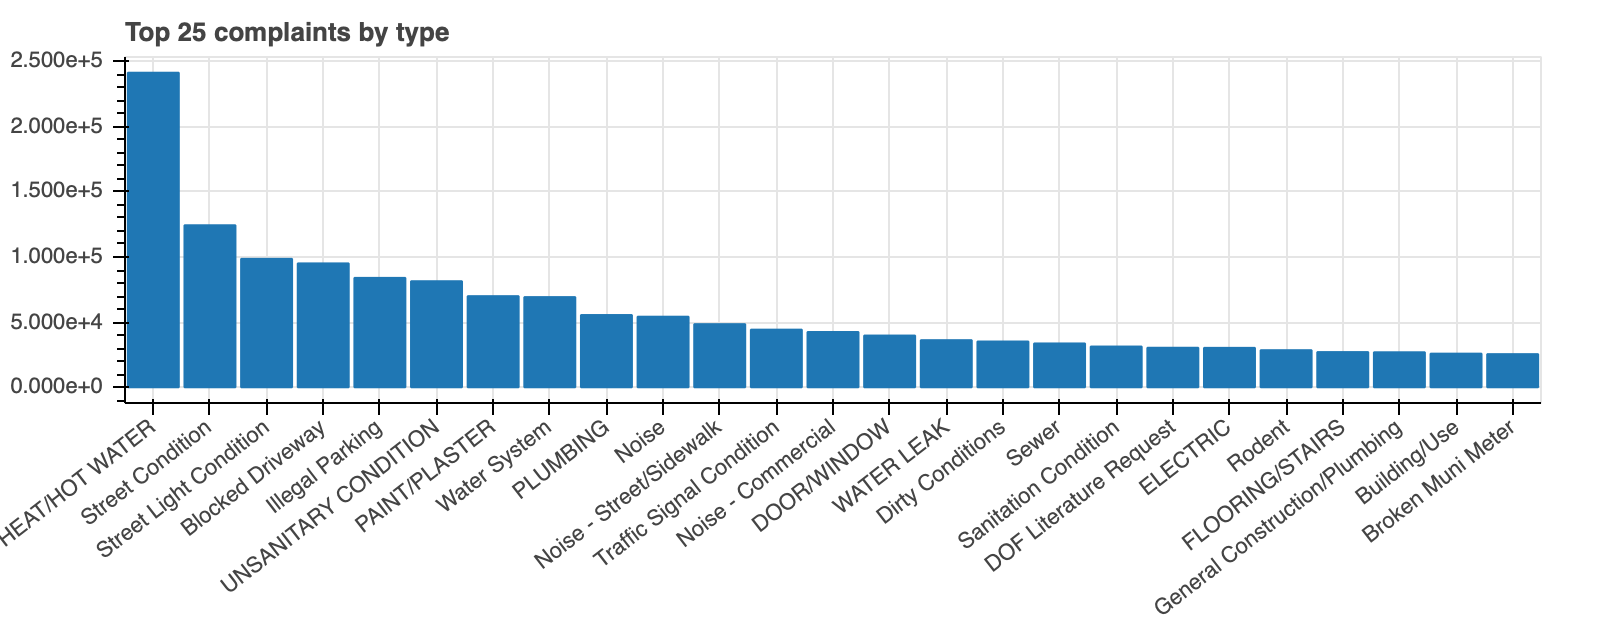
\includegraphics[scale=0.3]{top25complaints}

Heat/Hot Water comes out as the most common type of complaint.

\subsection{Top 10 cities with the largest number of complaints?}
Let's select the top 10 cities which have recorded the maximum number of complaints. As there are some rows which have None in the City, it is necessary to filter them out.
\begin{verbatim}
SELECT City AS name, COUNT(*) AS freq
    FROM data
    WHERE name <> 'None'
    GROUP BY name COLLATE NOCASE
    ORDER BY -freq
    LIMIT 10
\end{verbatim}

\begin{center}
 \begin{tabular}{||c c||}
 \hline
 name & freq \\ [0.5ex]
 \hline\hline
BROOKLYN    & 579363 \\
NEW YORK    & 385655 \\
BRONX   & 342533 \\
STATEN ISLAND   & 92509 \\
Jamaica & 46683 \\
Flushing    & 35504 \\
ASTORIA & 31873 \\
Ridgewood   & 21618 \\
Woodside    & 15932 \\
Corona  & 15740 \\ [1ex]
 % 5 & 88 & 788 & 6344 \\ [1ex]
 \hline
\end{tabular}
\end{center}

\subsection{What the number of complaints by type and by city for the top 7 cities?}

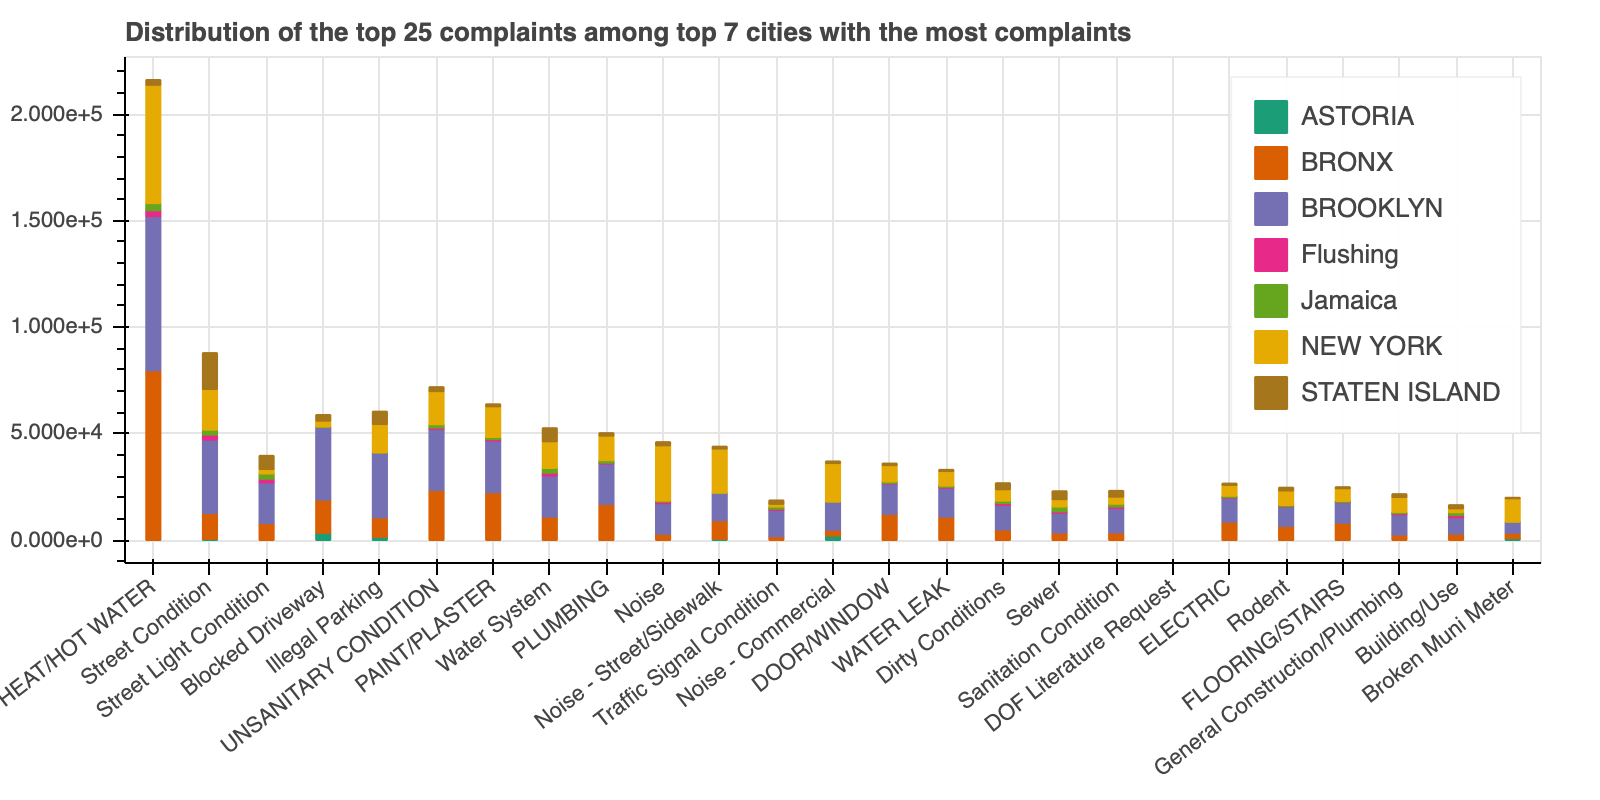
\includegraphics[scale=0.3]{topcomplaintsfortop7cities}

\subsection{What is the distribution of complaints by hour of day?}
\begin{verbatim}
SELECT strftime ('%H', CreatedDate) AS hour, COUNT(*) AS count
    FROM data
    GROUP BY hour
\end{verbatim}

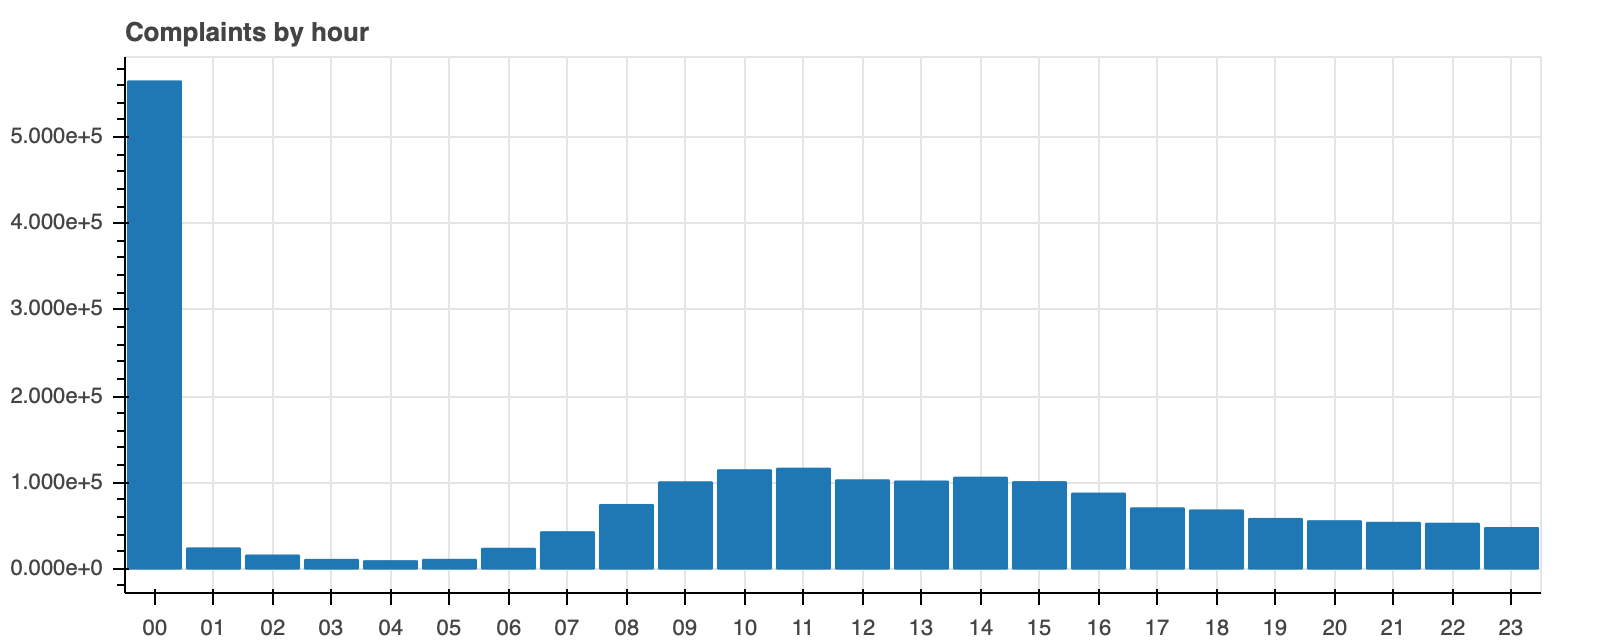
\includegraphics[scale=0.3]{complaintsbyhour}


An unusual aspect of this data is the excessively large number of reports associated with hour 0 (midnight up to but excluding 1 am). The reason is that there are some complaints that are dated but with no associated time, which was recorded in the data as exactly 00:00:00.000 as can be verified by the following SQL query:

\begin{verbatim}
SELECT COUNT(*)
    FROM data
    WHERE strftime ('%H:%M:%f', CreatedDate) = '00:00:00.000'

--- Result --

COUNT(*)
532285
\end{verbatim}


\subsection{What is the most common hour for noise complaints?}
A "noise complaint" is considered to be any complaint string containing the word noise. All dates without an associated time, i.e., a timestamp of 00:00:00.000 have been filtered out.

\begin{verbatim}
SELECT strftime ('%H', CreatedDate) AS hour, COUNT(*) as count
    FROM data
    WHERE strftime ('%H:%M:%f', CreatedDate) <>'00:00:00.000'
    AND ComplaintType LIKE '%noise%'
    GROUP BY hour
\end{verbatim}

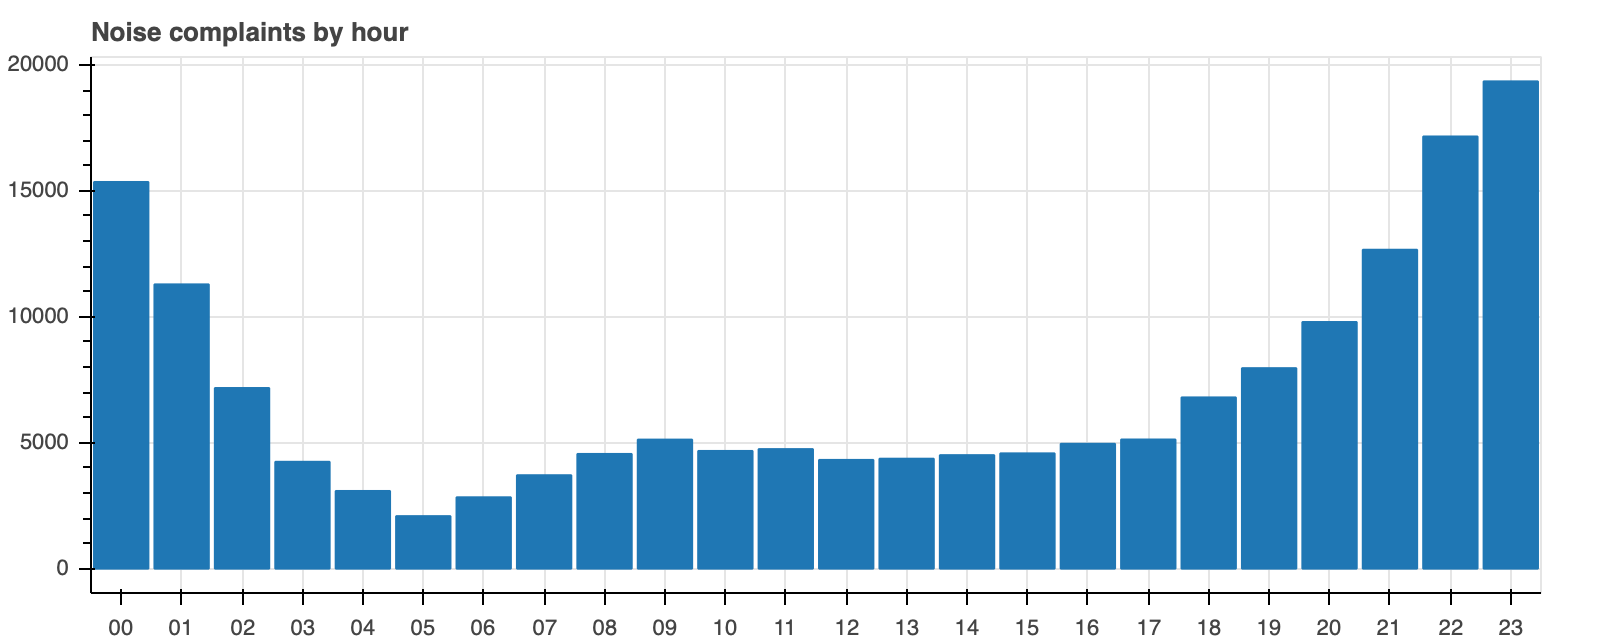
\includegraphics[scale=0.3]{noisecomplaintsbyhour}

function \cite{nycdatafull}.


% Bibliography:
\begin{thebibliography}{9}
\bibitem{latexcompanion}
Michel Goossens, Frank Mittelbach, and Alexander Samarin.
\textit{The \LaTeX\ Companion}.
Addison-Wesley, Reading, Massachusetts, 1993.

\bibitem{einstein}
Albert Einstein.
\textit{Zur Elektrodynamik bewegter K{\"o}rper}. (German)
[\textit{On the electrodynamics of moving bodies}].
Annalen der Physik, 322(10):891–921, 1905.

\bibitem{nycdatafull}
NYC Open Data
\\\texttt{https://nycopendata.socrata.com/Social-Services/311-Service-Requests\\-from-2010-to-Present/erm2-nwe9}


\bibitem{plotly}
Big data analytics using python and sqlite on NYC's 311 complaints since 2003.
\\\texttt{https://plot.ly/ipython-notebooks/big-data-\\analytics-with-pandas-and-sqlite/}

\bibitem{subset}
NYC Open Data
\\\texttt{https://onedrive.live.com/download?cid=FD520DDC6BE92730\&resid\\=FD520DDC6BE92730\%21616\&authkey=AEeP\_4E1uh-vyDE}


\end{thebibliography}

\end{document}


%% --- END OF FILE
